\section{Results}
\label{sec:results}

\subsection{Straight Wire Segment}
\begin{figure}[htbp]
 \centering
 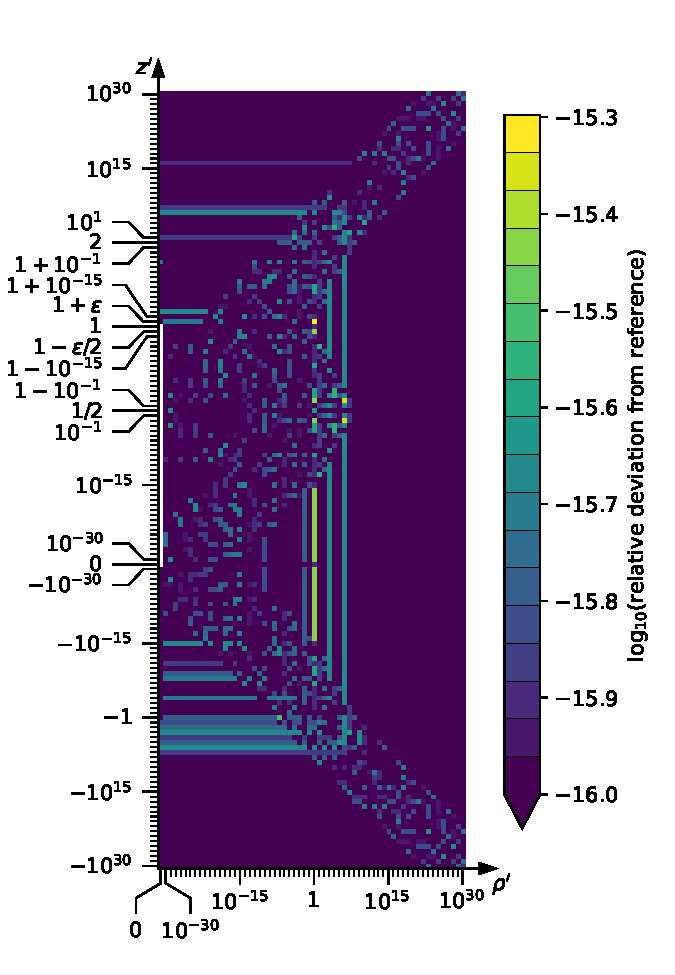
\includegraphics[height=\textwidth]{img/StraightWireSegment_A_z_Java.pdf}
 \caption{$\tilde{A}_z$ of straight wire segment: Comparison of the Java implementation against the reference data.}
 \label{fig:StraightWireSegment_A_z_Java}
\end{figure}
\begin{figure}[htbp]
 \centering
 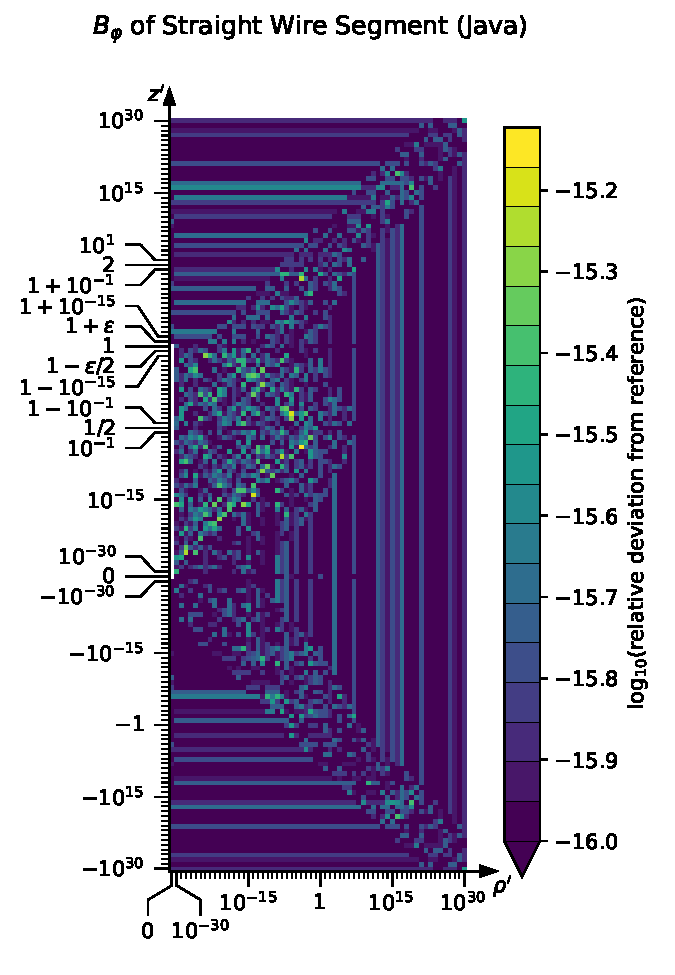
\includegraphics[height=\textwidth]{img/StraightWireSegment_B_phi_Java.pdf}
 \caption{$\tilde{B}_\varphi$ of straight wire segment: Comparison of the Java implementation against the reference data.}
 \label{fig:StraightWireSegment_B_phi_Java}
\end{figure}

\subsection{Circular Wire Loop}
\begin{figure}[htbp]
 \centering
 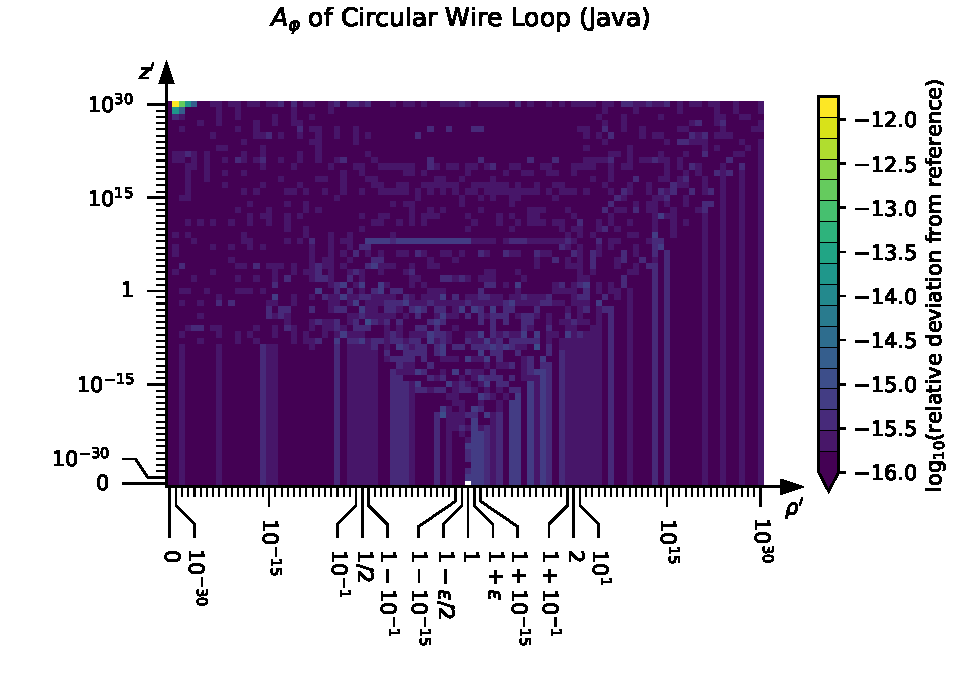
\includegraphics[width=0.8\textwidth]{img/CircularWireLoop_A_phi_Java.pdf}
 \caption{$\tilde{A}_\varphi$ of circular wire loop: Comparison of the Java implementation against the reference data.}
 \label{fig:CircularWireLoop_A_phi_Java}
\end{figure}
\begin{figure}[htbp]
 \centering
 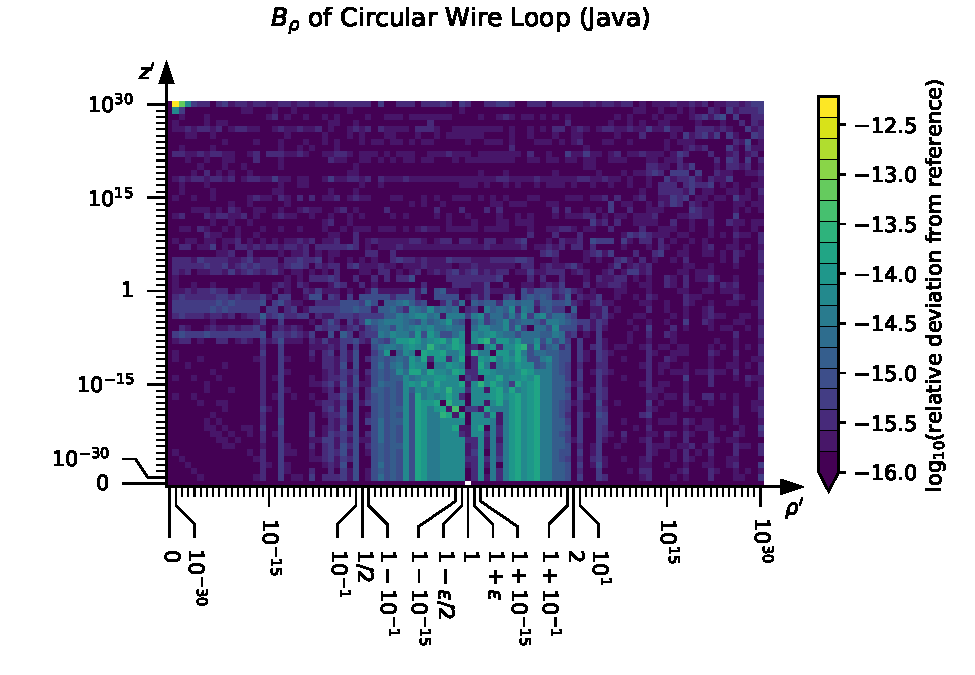
\includegraphics[width=0.8\textwidth]{img/CircularWireLoop_B_rho_Java.pdf}
 \caption{$\tilde{B}_\rho$ of circular wire loop: Comparison of the Java implementation against the reference data.}
 \label{fig:CircularWireLoop_B_rho_Java}
\end{figure}
\begin{figure}[htbp]
 \centering
 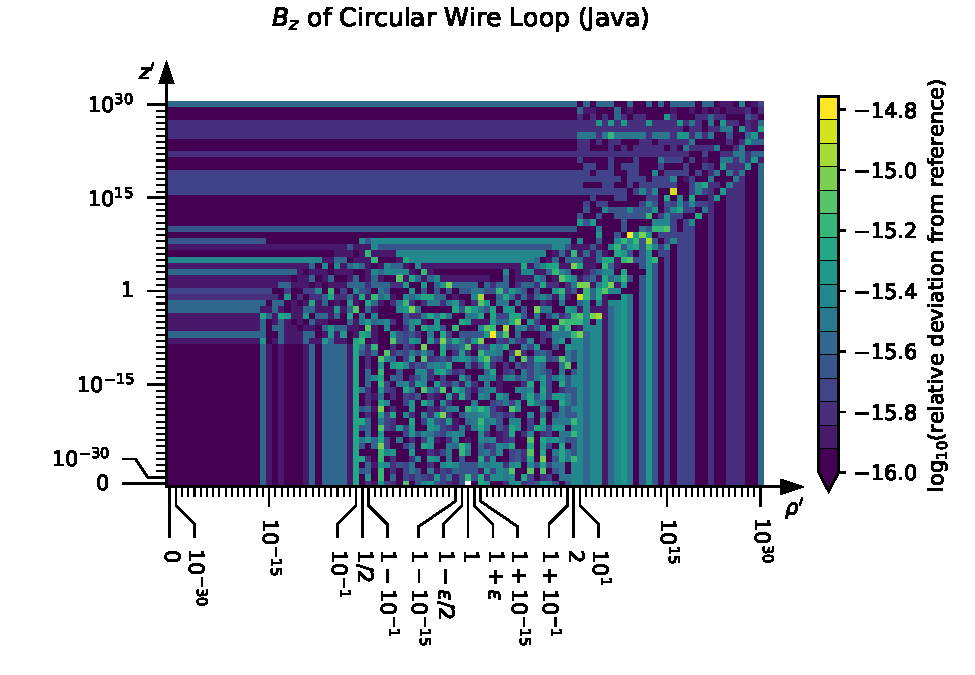
\includegraphics[width=0.8\textwidth]{img/CircularWireLoop_B_z_Java.pdf}
 \caption{$\tilde{B}_z$ of circular wire loop: Comparison of the Java implementation against the reference data.}
 \label{fig:CircularWireLoop_B_z_Java}
\end{figure}

\subsection{Further tests}

A second-order correction to the polygon approximation
for a circular wire loop~\cite{mcgreivy_2021} was tested.
Second-order iterative Kahan-Babuska summation~\cite{klein_2006} had to be used
to achive convergence down to numerical accuracy.

